%======================================================================
\section{El panorama en una página}
%======================================================================

\paragraph{La pregunta.} Un motor térmico microscópico tiene tres cosas que nos importan:
\begin{itemize}
\item su \textbf{potencia} media $P$ (cuánto trabajo entrega por unidad de tiempo),
\item su \textbf{eficiencia} $\eta$ (qué fracción del calor absorbido convierte en trabajo), o
  equivalentemente su \textbf{producción de entropía} $\Sigma$ (cuánto disipa),
\item sus \textbf{fluctuaciones de potencia} $\Delta P$ (qué tan irregular es la entrega).
\end{itemize}
No se pueden optimizar las tres a la vez: hay un compromiso. El conjunto de los mejores
compromisos es el \textbf{frente de Pareto}.

\paragraph{La práctica habitual.} Para encontrar el frente, muchos trabajos maximizan una
\emph{figura de mérito lineal}, por ejemplo $F = aP + b\eta - c\,\Delta P$, y barren los pesos
$(a,b,c)$. Cada elección de pesos da un motor óptimo; juntándolos se espera obtener el frente.

\paragraph{El problema.} Una suma ponderada solo puede encontrar los puntos del frente que están en
su envolvente convexa (los \emph{puntos soportados}). Si el frente tiene partes no convexas, la suma
ponderada no las ve, \emph{con ningún peso}.

\paragraph{Lo que mostramos.}
\begin{enumerate}
\item Si el frente satura la TUR (la cota de precisión que impone la segunda ley) y es una superficie
  (potencia y eficiencia se ajustan por separado), entonces en las variables $(P,\eta,\Delta P)$ el
  frente es una \textbf{silla de montar}: ningún punto interior es soportado.
\item Los \emph{mismos motores}, descritos con $(P,\Delta P,\Sigma)$, forman una superficie
  \textbf{convexa} (un ``tazón''): todos los puntos son soportados.
\item En un motor de Otto de un qubit, que satura la TUR, la suma ponderada con $\eta$ alcanza solo
  el $11\%$ del frente y pierde en mediana un $14\%$ en algún objetivo; con $\Sigma$ no pierde nada en
  la mediana.
\item En respuesta lineal (cerca del equilibrio) el frente es una curva y la suma ponderada funciona;
  con control muy libre la TUR se rompe y la silla desaparece. El efecto está ligado a la saturación.
\end{enumerate}

\begin{idea}
Elegir $\eta$ o $\Sigma$ como objetivo parece una cuestión de gusto, porque a potencia fija
maximizar una es minimizar la otra. Pero la relación entre ellas es no lineal, y una
transformación no lineal de coordenadas puede convertir una superficie convexa en una silla. La
suma ponderada es sensible a esa diferencia; la dominancia de Pareto no.
\end{idea}

\paragraph{Cómo leer esta guía.} Las secciones 2--5 son física (lo que verías en un curso de
termodinámica y mecánica estadística, aplicado a un qubit). Las secciones 6--9 son el resultado. Las
secciones 10--13 son los números, los algoritmos y el código. La sección 14 tiene ejercicios con
soluciones. Unidades: $\hbar = k_B = 1$ en todo el texto.

%======================================================================
\section{Un qubit en contacto con un baño térmico}
%======================================================================

\subsection{El sistema de dos niveles}

Un qubit es el sistema cuántico más simple: dos estados, que llamamos fundamental ($s=0$, energía
$0$) y excitado ($s=1$, energía $\omega$). La diferencia de energía $\omega$ es la \textbf{brecha}
(\emph{gap}). En un qubit superconductor (un transmón, por ejemplo) la brecha se controla desde
afuera con un flujo magnético; por eso tiene sentido pensar en $\omega$ como un parámetro que el
experimentador mueve, igual que el pistón de un motor mueve el volumen.

Como solo hay dos estados, el estado estadístico del qubit (sin coherencias) queda descrito por un
solo número: la \textbf{población excitada} $p$, la probabilidad de encontrarlo en $s=1$.

\subsection{Equilibrio: la distribución de Gibbs}

En equilibrio con un baño a temperatura $T$, el ensamble canónico da
\begin{equation}
p_{\mathrm{eq}} = \frac{e^{-\omega/T}}{1 + e^{-\omega/T}} = \frac{1}{1+e^{\omega/T}} \equiv a(\omega,T).
\label{eq:gibbs}
\end{equation}
Es la misma forma que la distribución de Fermi--Dirac (con potencial químico nulo), porque un nivel
que está ocupado o vacío es matemáticamente lo mismo que un qubit excitado o no. La población
excitada depende solo del cociente $\omega/T$: brecha grande o baño frío $\Rightarrow$ $a \to 0$;
brecha chica o baño caliente $\Rightarrow$ $a \to 1/2$ (Fig.~\ref{fig:poblacion}).

\begin{figure}[h]
\centering
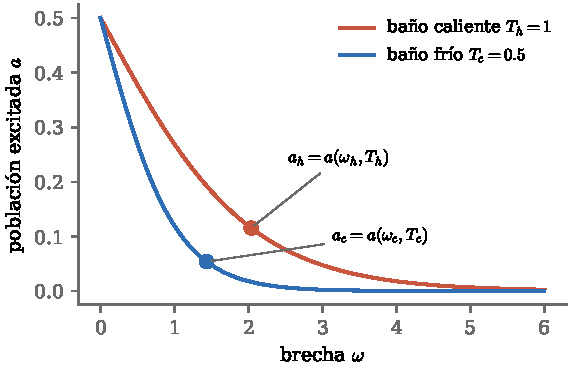
\includegraphics[width=0.62\linewidth]{figs/poblacion.pdf}
\caption{Población excitada de equilibrio $a(\omega,T)$ para los dos baños del proyecto
($T_h = 1$, $T_c = 0.5$). Los puntos marcan las brechas del motor de potencia máxima
($\omega_h = 2.04$, $\omega_c = 1.43$): aunque $\omega_h > \omega_c$, el baño caliente deja más
población excitada, $a_h > a_c$. Esa desigualdad es lo que hace funcionar el motor.}
\label{fig:poblacion}
\end{figure}

\subsection{Fuera del equilibrio: la ecuación maestra}

Si el qubit no está en equilibrio, el baño lo empuja hacia él. El modelo más simple es una
\textbf{ecuación maestra} con tasas de excitación $k_+$ y de decaimiento $k_-$:
\begin{equation}
\dot p = k_+(1-p) - k_-\,p .
\end{equation}
Para que el estado estacionario sea el de Gibbs, las tasas deben cumplir \textbf{balance detallado},
$k_+/k_- = e^{-\omega/T}$. Definiendo la tasa total $\gamma = k_+ + k_-$, la ecuación queda
\begin{equation}
\dot p = -\gamma\,\bigl(p - a(\omega,T)\bigr)
\qquad\Longrightarrow\qquad
p(t) = a + \bigl(p(0) - a\bigr)e^{-\gamma t}.
\label{eq:relax}
\end{equation}
La población relaja exponencialmente hacia $a$ con tiempo característico $1/\gamma$. En el proyecto
$\gamma = 1$, así que los tiempos están medidos en unidades de $1/\gamma$.

\subsection{La matriz de transición de un contacto}

Para la estadística necesitamos más que $p$: necesitamos la probabilidad de \emph{saltar} de un
estado a otro durante un contacto de duración $\tau$. Con $x = e^{-\gamma\tau}$ y la
ec.~\eqref{eq:relax}:
\begin{itemize}
\item si empieza en $s=0$ ($p(0)=0$), termina excitado con probabilidad $a(1-x)$;
\item si empieza en $s=1$ ($p(0)=1$), termina excitado con probabilidad $a + (1-a)x$, es decir,
  termina abajo con probabilidad $(1-a)(1-x)$.
\end{itemize}
Eso define la matriz estocástica (filas: estado inicial; columnas: estado final)
\begin{equation}
M = \begin{pmatrix} 1 - a(1-x) & a(1-x) \\ (1-a)(1-x) & 1 - (1-a)(1-x)\end{pmatrix},
\qquad \det M = x .
\label{eq:M}
\end{equation}
Esto es \code{relaxation\_matrix} en \code{otto/model.py}. Que $\det M = x$ (no depende de $a$)
será importante más adelante.

%======================================================================
\section{El ciclo de Otto cuántico}
%======================================================================

\subsection{Los cuatro tramos}

El ciclo de Otto de un motor a gasolina tiene dos adiabáticas (compresión y expansión) y dos
isocoras (calentamiento y enfriamiento a volumen fijo). En el Otto cuántico, la brecha $\omega$ hace
el papel del volumen:
\begin{enumerate}
\item \textbf{Isocora caliente.} Brecha fija $\omega_h$, contacto con el baño caliente $T_h$ durante
  $\tau_h$. La población sube de $p_2$ a $p_1$.
\item \textbf{Adiabática (quench).} Se desconecta el baño y se cambia la brecha $\omega_h\to\omega_c$
  en un tiempo $\tau_q$, tan rápido que la población no cambia.
\item \textbf{Isocora fría.} Brecha $\omega_c$, contacto con el baño frío $T_c$ durante $\tau_c$. La
  población baja de $p_1$ a $p_2$.
\item \textbf{Adiabática de vuelta}, $\omega_c\to\omega_h$, otra vez a población fija.
\end{enumerate}

\subsection{Calor y trabajo: la primera ley microscópica}

La energía media del qubit es $E = \sum_s \varepsilon_s p_s = \omega\,p$. Su diferencial tiene dos
términos:
\begin{equation}
\dd E = \underbrace{\sum_s \varepsilon_s\,\dd p_s}_{\text{calor}} \;+\;
\underbrace{\sum_s p_s\,\dd\varepsilon_s}_{\text{trabajo}}
\;=\; \omega\,\dd p + p\,\dd\omega .
\end{equation}
Cambiar las \emph{probabilidades} con los niveles fijos es intercambiar calor con el baño; cambiar
los \emph{niveles} con las probabilidades fijas es hacer trabajo. Es exactamente la separación que
usa la termodinámica cuántica, y en el Otto los tramos la separan limpiamente
(Fig.~\ref{fig:ciclo}, izquierda):
\begin{align}
Q_h &= \omega_h\,(p_1 - p_2) &&\text{(calor absorbido del baño caliente)}\\
Q_c &= \omega_c\,(p_1 - p_2) &&\text{(calor entregado al baño frío)}\\
W   &= Q_h - Q_c = (\omega_h - \omega_c)(p_1 - p_2) &&\text{(trabajo extraído por ciclo)}
\end{align}

\begin{figure}[h]
\centering
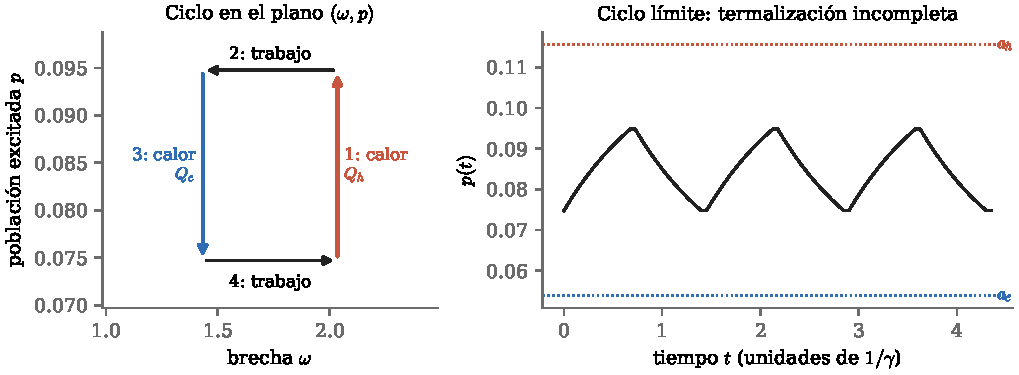
\includegraphics[width=\linewidth]{figs/ciclo.pdf}
\caption{Izquierda: el ciclo de Otto en el plano $(\omega,p)$ para el motor de potencia máxima; el
área encerrada es el trabajo $W$. Derecha: la población $p(t)$ durante tres ciclos. Nunca llega a
$a_h$ ni a $a_c$: la termalización es incompleta. Después de unos pocos ciclos el qubit entra en un
\emph{ciclo límite} y $p$ oscila entre $p_2$ y $p_1$.}
\label{fig:ciclo}
\end{figure}

\subsection{Eficiencia de Otto y la condición para ser motor}

Dividiendo,
\begin{equation}
\eta = \frac{W}{Q_h} = 1 - \frac{\omega_c}{\omega_h}.
\label{eq:etaotto}
\end{equation}
La eficiencia depende \emph{solo} del cociente de brechas $r = \omega_c/\omega_h$, no de los tiempos.
Para que el ciclo sea un motor ($W > 0$) necesitamos $p_1 > p_2$, lo que (como veremos) requiere
$a_h > a_c$:
\begin{equation}
\frac{1}{1+e^{\omega_h/T_h}} > \frac{1}{1+e^{\omega_c/T_c}}
\iff \frac{\omega_h}{T_h} < \frac{\omega_c}{T_c}
\iff r > \frac{T_c}{T_h}
\iff \eta < 1 - \frac{T_c}{T_h} = \etaC .
\end{equation}
La segunda ley aparece sola: el Otto nunca supera a Carnot. Por eso en el código la variable
$r$ vive en $[T_c/T_h,\,1]$: con $r = T_c/T_h$ se tiene $\eta = \etaC$ (pero potencia nula), y con
$r = 1$ se tiene $\eta = 0$.

\subsection{Tiempo finito: el ciclo límite}

Con contactos de duración finita, $x_h = e^{-\gamma\tau_h}$ y $x_c = e^{-\gamma\tau_c}$ son distintos
de cero y el qubit no termaliza. Aplicando \eqref{eq:relax} a cada contacto,
\begin{equation}
p_1 = a_h + (p_2 - a_h)x_h, \qquad p_2 = a_c + (p_1 - a_c)x_c .
\end{equation}
Resolviendo el sistema (ejercicio~\ref{ej:ciclolimite}):
\begin{equation}
\boxed{\;p_1 - p_2 = \frac{(a_h - a_c)(1-x_h)(1-x_c)}{1 - x_h x_c}\;}
\label{eq:dp}
\end{equation}
Esta fórmula lo explica casi todo:
\begin{itemize}
\item el signo lo pone $a_h - a_c$: hay motor si y solo si $r > T_c/T_h$;
\item los factores $(1-x)$ castigan los contactos cortos: si $\tau\to 0$, $x\to1$ y no hay
  intercambio de calor;
\item la potencia es $P = W/\tau_{\mathrm{ciclo}}$ con $\tau_{\mathrm{ciclo}} = \tau_h + \tau_c + 2\tau_q$,
  que castiga los contactos largos.
\end{itemize}
Entre ambos extremos hay un óptimo: el \textbf{compromiso potencia--eficiencia}.

\begin{ejemplo}[El motor de potencia máxima]
Con $T_h = 1$, $T_c = 0.5$, $\gamma = 1$ y $\tau_q = 0.05$, el máximo de potencia está en
$\omega_h \approx 2.035$, $r \approx 0.704$ ($\omega_c \approx 1.433$), $\tau_h \approx \tau_c \approx 0.675$.
Ahí:
\begin{center}
\begin{tabular}{lll}
\toprule
$a_h = 0.116$, $a_c = 0.054$ & $p_1 = 0.0948$, $p_2 = 0.0747$ & $\tau_{\mathrm{ciclo}} = 1.450$ \\
$W = 0.0121$ por ciclo & $P = 0.00833$ & $\eta = 0.296$ \\
$\Delta P = 0.0126$ & $\Sigma = 0.0115$ & $\xi = 0.96$ \\
\bottomrule
\end{tabular}
\end{center}
La eficiencia a potencia máxima, $0.296$, es casi la de \textbf{Curzon--Ahlborn},
$1-\sqrt{T_c/T_h} = 0.293$. Fue la primera verificación de que el modelo se comporta como un motor
físico razonable. ($\Delta P$, $\Sigma$ y $\xi$ se definen en las secciones siguientes.)
\end{ejemplo}

%======================================================================
\section{Termodinámica estocástica: el trabajo fluctúa}
%======================================================================

\subsection{Un solo qubit no tiene ``población 0.09''}

Hasta aquí usamos promedios. Pero un qubit individual está, en cada instante, arriba o abajo. Al
hacer el primer quench, si está excitado ($s_1 = 1$) entrega $\Delta\omega = \omega_h - \omega_c$ de
trabajo; si está abajo, nada. En el segundo quench, si está excitado ($s_2 = 1$) hay que pagar
$\Delta\omega$. El trabajo de un ciclo es una \textbf{variable aleatoria}:
\begin{equation}
w = \Delta\omega\,(s_1 - s_2) \in \{-\Delta\omega,\ 0,\ +\Delta\omega\}.
\end{equation}
Su media es $\langle w\rangle = \Delta\omega(p_1 - p_2) = W$, pero en un ciclo dado puede ser
negativa. Esta es la idea central de la \emph{termodinámica estocástica}: calor, trabajo y entropía
se definen trayectoria por trayectoria y fluctúan; las leyes de la termodinámica valen para los
promedios (y, más finamente, para las distribuciones).

\subsection{Qué queremos medir}

Tras $n$ ciclos el trabajo acumulado es $W_n = \sum_{k=1}^n w_k$. Para $n$ grande,
\begin{equation}
\langle W_n\rangle \simeq n\,\langle w\rangle, \qquad
\operatorname{Var}(W_n) \simeq n\,v ,
\end{equation}
y definimos la \textbf{potencia} y las \textbf{fluctuaciones de potencia} como tasas:
\begin{equation}
P = \frac{\langle w\rangle}{\tau_{\mathrm{ciclo}}}, \qquad
\Delta P = \lim_{t\to\infty}\frac{\operatorname{Var}(W_t)}{t} = \frac{v}{\tau_{\mathrm{ciclo}}} .
\end{equation}
$\Delta P$ es un coeficiente de difusión: mide cuánto se abre el abanico de trayectorias
(Fig.~\ref{fig:tray}).

\begin{figure}[h]
\centering
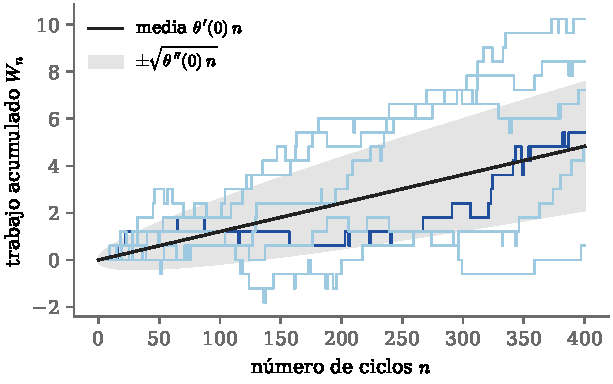
\includegraphics[width=0.66\linewidth]{figs/trayectorias.pdf}
\caption{Seis trayectorias simuladas del trabajo acumulado en el motor de potencia máxima. Todas
crecen en promedio con pendiente $\theta'(0)$, pero se separan como $\sqrt{n}$; la banda gris es
$\pm\sqrt{\theta''(0)\,n}$. $P$ es la pendiente por unidad de tiempo; $\Delta P$ es el ancho del
abanico por unidad de tiempo.}
\label{fig:tray}
\end{figure}

\paragraph{La trampa: correlaciones.} Uno estaría tentado de calcular $v = \operatorname{Var}(w)$ de
un ciclo. Pero los ciclos están correlacionados: si un ciclo termina con el qubit excitado, el
siguiente empieza excitado. Entonces $\operatorname{Var}(W_n) \neq n\operatorname{Var}(w)$; hay que
sumar todas las covarianzas entre ciclos. La herramienta que hace esto de una vez es la estadística
de conteo completa.

\subsection{Estadística de conteo completa y la matriz inclinada}

La \textbf{función generadora de momentos} del trabajo acumulado es
$\langle e^{\chi W_n}\rangle$. Como el qubit es una cadena de Markov, esa suma sobre trayectorias
se puede escribir como un producto de matrices. En cada ciclo:
\begin{itemize}
\item se pasa del estado $s$ (al inicio) a $s_1$ con $M^h$, y se acumula el factor
  $e^{\chi\Delta\omega s_1}$ del primer quench;
\item se pasa de $s_1$ a $s'$ con $M^c$, y se acumula $e^{-\chi\Delta\omega s'}$ del segundo quench.
\end{itemize}
Eso define la \textbf{matriz inclinada} (\emph{tilted matrix}) de un ciclo:
\begin{equation}
\mathcal{T}(\chi)_{s s'} = \sum_{s_1\in\{0,1\}} M^h_{s s_1}\,e^{\chi\Delta\omega s_1}\,M^c_{s_1 s'}\,e^{-\chi\Delta\omega s'} ,
\qquad
\langle e^{\chi W_n}\rangle = \pi^{\top}\,\mathcal{T}(\chi)^n\,\mathbf{1} .
\end{equation}
Para $\chi = 0$ es la matriz de transición de un ciclo completo (estocástica, autovalor máximo
$1$). Para $n$ grande, $\mathcal{T}^n$ está dominada por su mayor autovalor $\lambda(\chi)$:
\begin{equation}
\langle e^{\chi W_n}\rangle \asymp \lambda(\chi)^n
\quad\Longrightarrow\quad
\theta(\chi) \equiv \lim_{n\to\infty}\frac{1}{n}\ln\langle e^{\chi W_n}\rangle = \ln\lambda(\chi).
\end{equation}
$\theta$ es la \textbf{función generadora de cumulantes escalada}. Sus derivadas en $\chi=0$ dan los
cumulantes por ciclo, \emph{con todas las correlaciones incluidas}:
\begin{equation}
\langle w\rangle = \theta'(0), \qquad v = \theta''(0).
\end{equation}

\begin{idea}[Analogía con el ensamble canónico]
$\theta(\chi)$ cumple para el trabajo el papel que $\ln Z(\beta)$ cumple para la energía: derivarla
da la media y la varianza. Y, como en mecánica estadística, la probabilidad de observar un trabajo
por ciclo atípico $w$ decae como $e^{-n I(w)}$, donde la ``función de tasa'' $I$ es la
\emph{transformada de Legendre} de $\theta$ (teoría de grandes desviaciones). Volveremos a encontrar
una transformada de Legendre en el resultado central (sección~\ref{sec:legendre}).
\end{idea}

\subsection{Forma cerrada (por qué el cálculo es exacto)}

Una matriz $2\times2$ tiene autovalores que dependen solo de su traza $t(\chi)$ y su determinante
$D(\chi)$:
\begin{equation}
\lambda(\chi) = \tfrac12\Bigl(t + \sqrt{t^2 - 4D}\Bigr).
\end{equation}
\textbf{El determinante no depende de $\chi$.} Como $\det(AB) = \det A\det B$ y los factores
$e^{\pm\chi\Delta\omega s}$ son matrices diagonales que se cancelan en el determinante,
$D = \det M^h\det M^c = x_h x_c$ (por la ec.~\eqref{eq:M}). La traza sí depende de $\chi$:
\begin{equation}
t(\chi) = c_0 + c_+e^{\chi\Delta\omega} + c_-e^{-\chi\Delta\omega},\qquad
c_+ = M^h_{01}M^c_{10},\quad c_- = M^h_{10}M^c_{01}.
\end{equation}
($c_+$: subir en el baño caliente y bajar en el frío, un ciclo ``productivo''; $c_-$: lo contrario.)
Derivando implícitamente $\lambda^2 - t\lambda + D = 0$ y usando $\lambda(0) = 1$, $t(0) = 1 + D$:
\begin{equation}
\lambda'(0) = \frac{t'(0)}{1-D},\qquad
\lambda''(0) = \frac{t''(0)}{1-D} - \frac{2D\,t'(0)^2}{(1-D)^3},
\end{equation}
con $t'(0) = \Delta\omega(c_+ - c_-)$ y $t''(0) = \Delta\omega^2(c_+ + c_-)$. Finalmente
$\theta'(0) = \lambda'(0)$ y $\theta''(0) = \lambda''(0) - \lambda'(0)^2$. Esto es literalmente lo
que hace \code{cycle\_statistics}. Se puede comprobar que $\theta'(0) = \Delta\omega(p_1 - p_2)$,
de acuerdo con la ec.~\eqref{eq:dp}.

\paragraph{Validación.} \code{monte\_carlo\_work} simula miles de qubits saltando con números
aleatorios y estima media y varianza por fuerza bruta. Coinciden con $\theta'(0)$ y $\theta''(0)$
dentro del error estadístico, y las derivadas analíticas coinciden con diferencias finitas de
$\theta$. Esa es la base de confianza de todo lo demás.

%======================================================================
\section{Producción de entropía y la relación de incertidumbre termodinámica}
%======================================================================

\subsection{Producción de entropía}

La entropía del qubit vuelve a su valor inicial en cada ciclo, así que toda la entropía producida
termina en los baños. Por unidad de tiempo:
\begin{equation}
\Sigma = \frac{1}{\tau_{\mathrm{ciclo}}}\left(\frac{Q_c}{T_c} - \frac{Q_h}{T_h}\right) \;\ge\; 0 .
\end{equation}
Es la segunda ley. Usando $Q_h = P\tau/\eta$ y $Q_c = Q_h - W$ (ejercicio~\ref{ej:sigma}):
\begin{equation}
\boxed{\;\Sigma = \frac{P\,(\etaC - \eta)}{\eta\,T_c}\;}
\qquad\Longleftrightarrow\qquad
\eta = \frac{\etaC\,P}{P + T_c\,\Sigma}.
\label{eq:sigma}
\end{equation}
Lectura: $\eta = \etaC$ si y solo si $\Sigma = 0$ (proceso reversible). A potencia fija, maximizar
$\eta$ y minimizar $\Sigma$ son lo mismo. Pero la relación entre ambas es \emph{no lineal}, y eso
será decisivo.

En el modelo de Otto, $\Sigma = (p_1 - p_2)\bigl(\omega_c/T_c - \omega_h/T_h\bigr)/\tau_{\mathrm{ciclo}}$,
que es positivo justamente cuando $r > T_c/T_h$.

\subsection{La relación de incertidumbre termodinámica (TUR)}

La TUR (Barato y Seifert 2015; Gingrich \emph{et al.} 2016) dice que \textbf{la precisión cuesta
disipación}. Para cualquier corriente $J_t$ (algo que se acumula en el tiempo, como el trabajo) de un
proceso de Markov estacionario,
\begin{equation}
\frac{\operatorname{Var}(J_t)}{\langle J_t\rangle^2}\;\ge\;\frac{2}{\Sigma\,t}.
\end{equation}
El lado izquierdo es el ruido relativo; para hacerlo pequeño hay que disipar mucho. Aplicada al
trabajo, con $\langle W_t\rangle = Pt$ y $\operatorname{Var}(W_t) = \Delta P\,t$:
\begin{equation}
\boxed{\;\Delta P\;\Sigma\;\ge\;2P^2\;}
\label{eq:tur}
\end{equation}
Sustituyendo \eqref{eq:sigma} se obtiene la forma de Pietzonka y Seifert (2018) para motores
(ejercicio~\ref{ej:tur}):
\begin{equation}
\eta \;\le\; \frac{\etaC}{1 + 2T_cP/\Delta P}.
\end{equation}
Es un compromiso a tres bandas: para acercarse a Carnot con potencia finita hay que aceptar
fluctuaciones grandes ($\Delta P\to\infty$).

\subsection{El cociente $\xi$ y la saturación}

Definimos
\begin{equation}
\xi = \frac{2P^2}{\Delta P\,\Sigma} = \frac{2T_c\,P\,\eta}{\Delta P\,(\etaC - \eta)} ,
\end{equation}
de modo que la TUR dice $\xi \le 1$. \textbf{Saturar} la TUR es tener $\xi = 1$: el motor es tan
regular como la segunda ley permite para su disipación. Esto define una superficie en el espacio
$(P,\eta,\Delta P)$:
\begin{equation}
\Delta P = g(P,\eta) \equiv \frac{2T_c\,\eta\,P}{\etaC - \eta}.
\label{eq:g}
\end{equation}

\paragraph{Resultado del proyecto.} En el Otto de un qubit, \emph{todo} el frente de Pareto está
sobre esa superficie: mediana $\xi = 0.996$, máximo $1.005$. Que haya puntos con $\xi$ apenas mayor
que 1 no es un error: la TUR está demostrada para procesos \emph{estacionarios}, y un motor cíclico
con forzamiento periódico puede violarla (Holubec y Ryabov 2018; Koyuk, Seifert y Pietzonka 2019).
Erdman \emph{et al.} (2023) ya habían notado la saturación en ciclos de Otto rápidos.
